\usetikzlibrary{patterns}


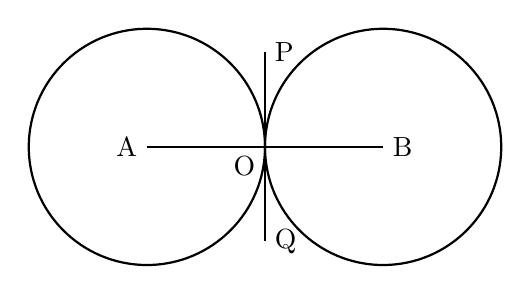
\begin{tikzpicture}[scale=1]

    % Define the coordinates for the centers of the two circles
    % They are horizontally aligned and tangent at the origin (0,0)
    \coordinate (A) at (-1.5, 0);
    \coordinate (B) at (1.5, 0);
    
    % Define the point of intersection/tangency
    \coordinate (O) at (0, 0);

    % Draw the two circles (assuming equal radius of 1.5 to make them tangent at origin)
    \draw[thick] (A) circle (1.5);
    \draw[thick] (B) circle (1.5);

    % Draw the horizontal line segment connecting center A and center B
    \draw[thick] (A) -- (B);

    % Draw the vertical common tangent line segment passing through O
    % The line does not extend beyond the top and bottom of the circles
    \draw[thick] (0, 1.2) -- (0, -1.2);

    % Label the center points exactly as shown in the image
    \node[left] at (A) {A};
    \node[right] at (B) {B};
    
    % Label the intersection point O (below and to the left of the center)
    \node[below left] at (O) {O};
    
    % Label the ends of the vertical tangent line P and Q
    \node[right] at (0, 1.2) {P};
    \node[right] at (0, -1.2) {Q};

\end{tikzpicture}